\documentclass[10pt, aspectratio=1610]{beamer}
\usepackage{amsmath, amsfonts}
\usepackage{multirow}
\usepackage{array}
\usepackage{tikz}
\usepackage{pgfplots}
\usepackage{subfig}
\usepackage{threeparttable}
\usepackage{glossaries}
\usepackage{xcolor}
\usepackage[utf8]{inputenc}


\usepackage[ruled, vlined, linesnumbered]{algorithm2e}
\usepackage{hyperref}

\usepackage{roboto}

%% Set colors for the presentation
\definecolor{t1}{RGB}{239, 35, 60} %red
\definecolor{t2}{RGB}{43, 45, 66} %dark grey
\definecolor{t3}{RGB}{141, 153, 174} % gray

\setbeamercolor{title}{fg=t2}
\setbeamercolor{frametitle}{fg=t2}
\setbeamercolor{subtitle}{fg=t2}
\setbeamercolor{section in toc}{fg=t2}
\setbeamercolor{subsection in toc}{fg=t2}
\setbeamercolor{caption}{fg=t2}
\setbeamercolor{caption name}{fg=t2}
\setbeamercolor{item}{fg=t2}
\setbeamercolor{itemize item}{fg=t1}
\setbeamercolor{enumerate item}{fg=t2}

\setbeamertemplate{itemize item}[circle]
\setbeamertemplate{navigation symbols}{}
\setbeamertemplate{section in toc}[sections numbered]
\setbeamertemplate{subsection in toc}[subsections numbered]

\usefonttheme{professionalfonts}

\setbeamerfont{title}{series=\bfseries}
\setbeamerfont{section in toc}{series=\bfseries}
\setbeamerfont{frametitle}{series=\bfseries}
\setbeamerfont{caption name}{series=\bfseries}

\usetikzlibrary{arrows.meta}
\usetikzlibrary{datavisualization.formats.functions}

% \mode<presentation>
\title{Technical Impacts on Voltage from Home EV Charging: 
A Case Study in Cusco, Peru}

\author[Derian Tairo]{Derian Carlos Tairo Garcia \\
    Erick Alberto Somocurcio Holguín}
\date{\today}

\begin{document}
    
\begin{frame}
    \titlepage
\end{frame}

\begin{frame}
    \frametitle{Table of Contents}
    \tableofcontents
\end{frame}
% \logo{
\includegraphics[height=1cm]{../Figures/unicamp_logo.png}}

\section{Introduction}
\subsection{Objectives}
\begin{frame}
    \frametitle{Objectives}
    \begin{itemize}%[<+->]
        \item Create a detailed database for OpenDSS 
        to simulate EVs connection.
        \item Simulated several scenarios of EVs connection.
        \item Analyze the technical impacts (Voltage magnitude) of 
        EVs on Cusco's electrical grid.
    \end{itemize}
\end{frame}
\subsection{Context}
\begin{frame}
    \frametitle{Substation Quencoro 138/10.5KV AMT QU02 - Cusco}
    \begin{figure}
        \includegraphics[width = 0.8\textwidth]{../Figures/SE QUENCORO_Operación.pdf}
    \end{figure}
\end{frame}

\begin{frame}
    \frametitle{AMT QU02 - SED022}
    \begin{figure}
        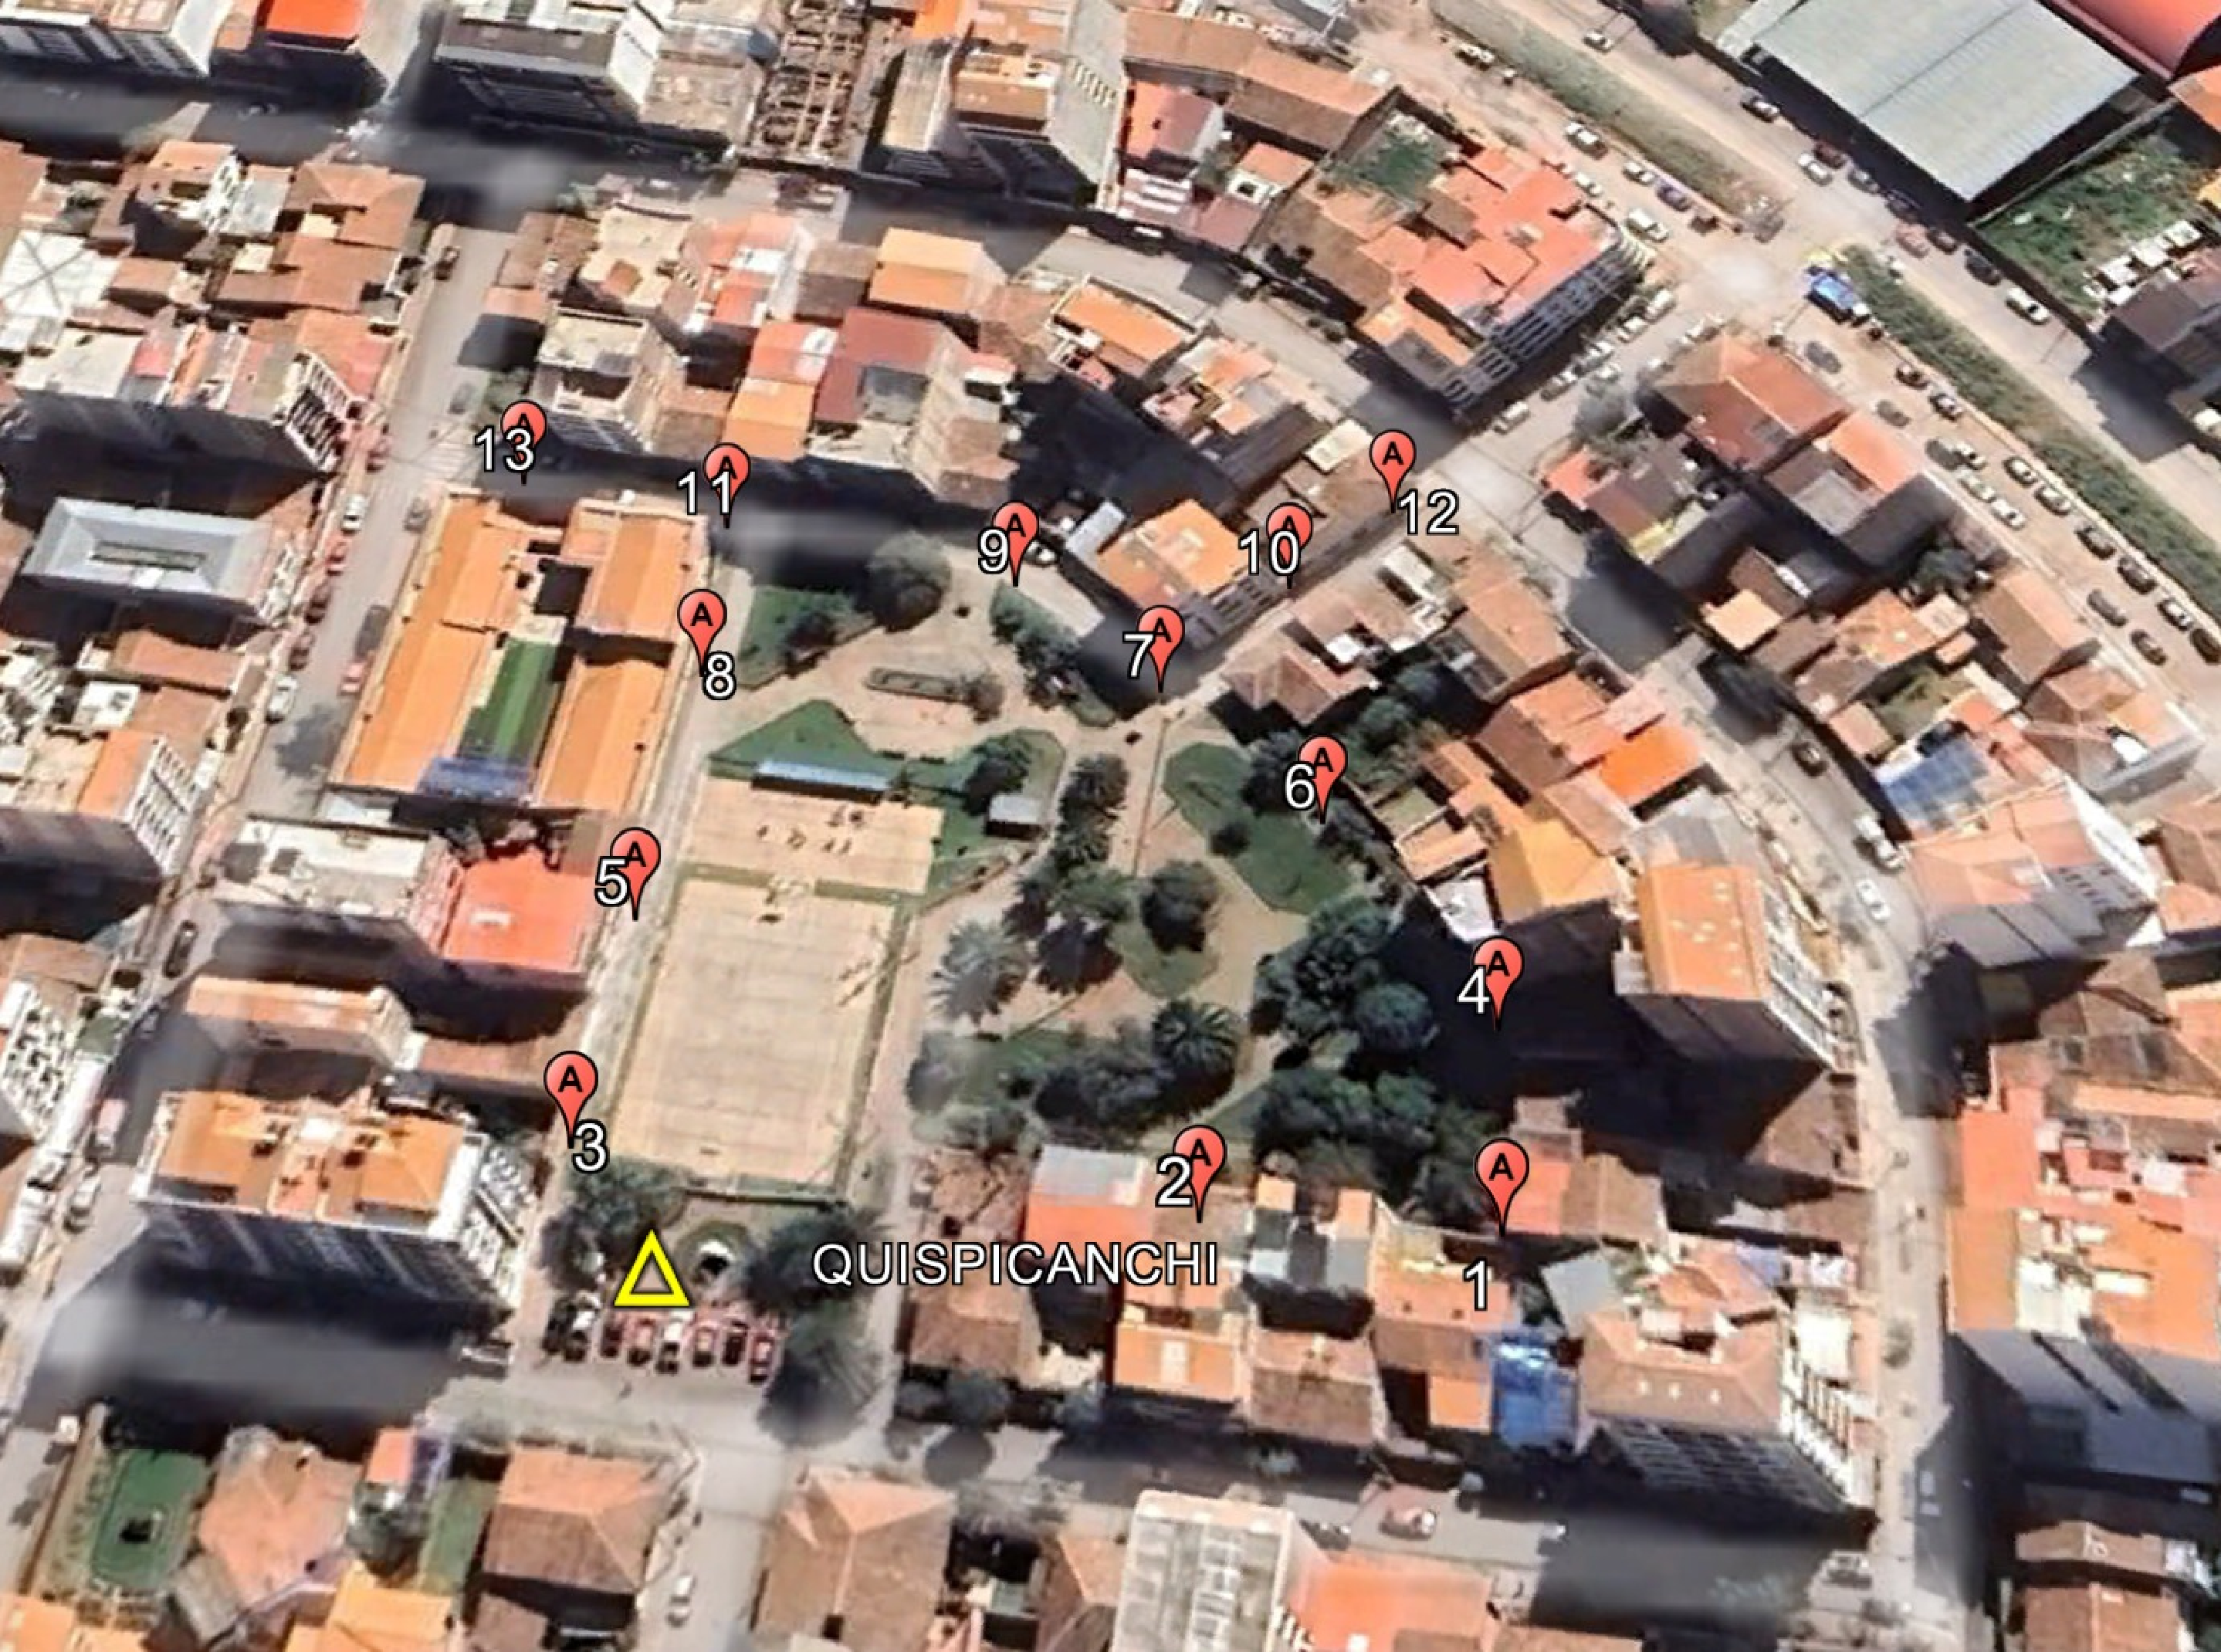
\includegraphics[width = 0.8\textwidth]{../Figures/casas.pdf}
    \end{figure}
\end{frame}


\section{Case Study}

\begin{frame}
    \frametitle{SED022 - Parameters}
    \begin{figure}
        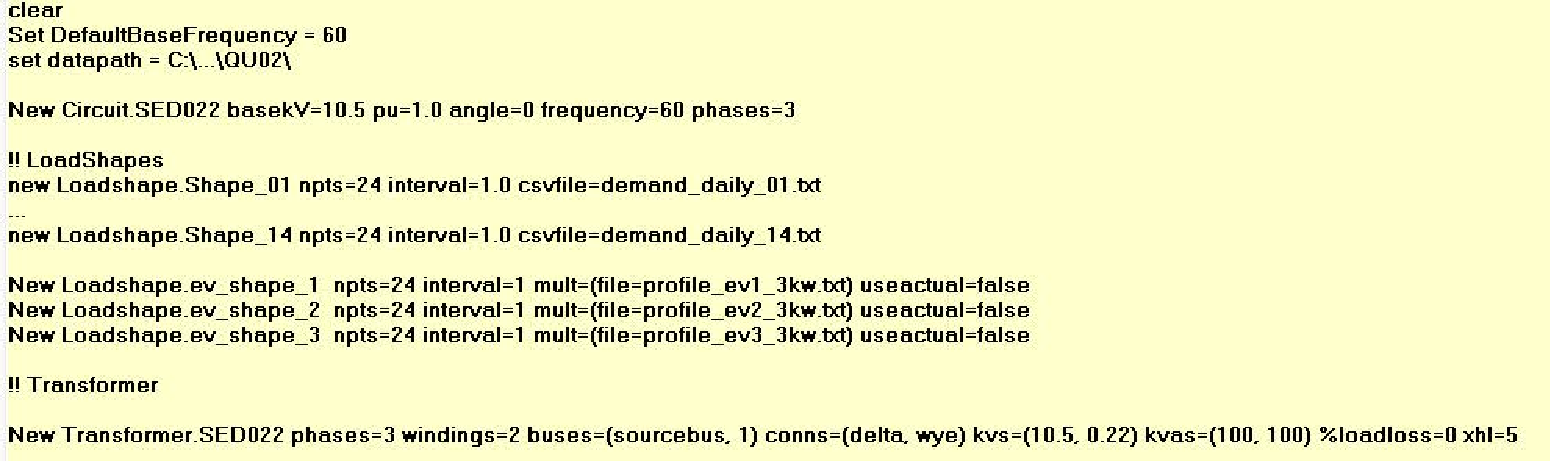
\includegraphics[width = \textwidth]{../Figures/code_1.pdf}
    \end{figure}
\end{frame}
\begin{frame}
    \frametitle{SED022 - Parameters}
    \begin{figure}
        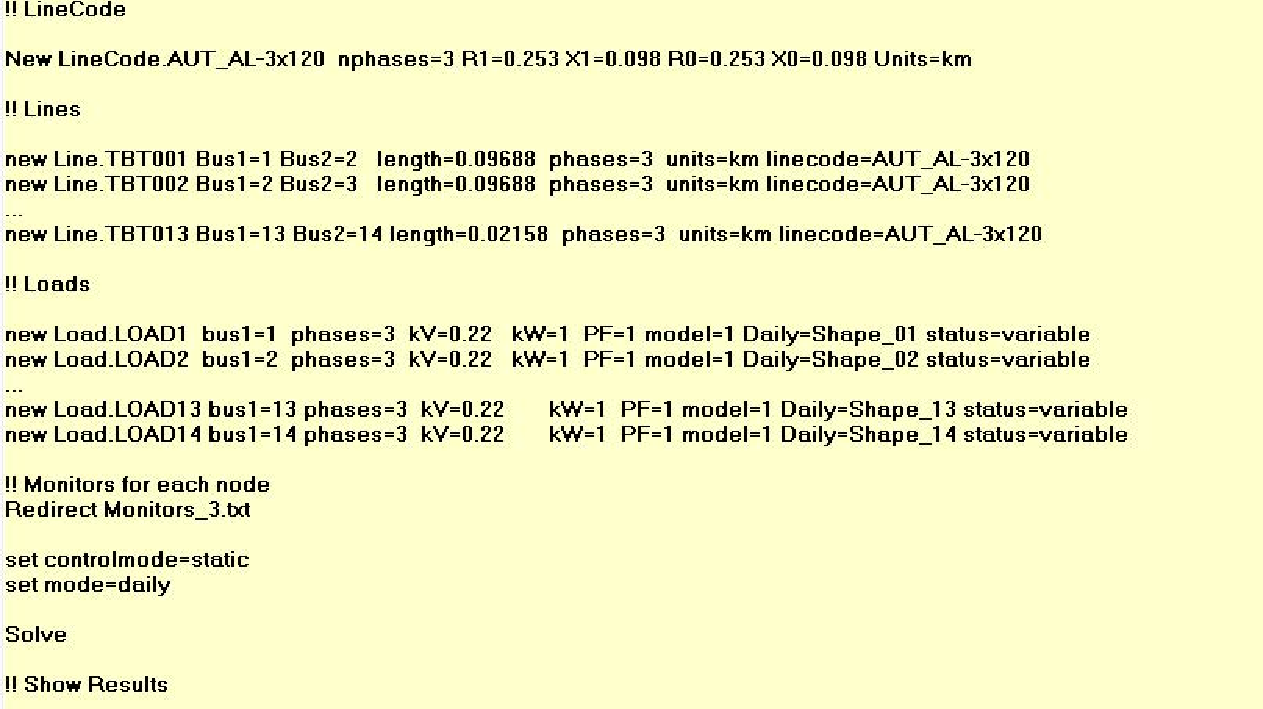
\includegraphics[width = \textwidth]{../Figures/code_2.pdf}
    \end{figure}
\end{frame}

% \begin{frame}
%     \frametitle{Case Study}
%     \framesubtitle{Load profiles for each node}

%     \begin{figure}
%             \begin{tikzpicture}[baseline]
%                 \begin{axis}[
%                 xlabel={Period time [h]},
%                 ylabel near ticks,
%                 xlabel near ticks,
%                 ylabel={Voltage [V]},
%                 % tick style = {line width = 0.5, color = lightgray, 
%                 %     major tick length=4pt,minor tick length=2pt,
%                 %     minor x tick num = 3, minor y tick num =1},
%                 % tick label style = {font=\small, xtick distance=4, 
%                 %     xticklabels={00:00, 00:00, 04:00, 08:00, 12:00, 16:00, 20:00}},
%                 % label style = {},
%                 legend style = {font=\footnotesize, at={(0.99,0.98)}, 
%                     legend cell align=left, line width=0.5pt, draw=lightgray},
%                 % % legend entries={High PV, Medium PV, Low PV, High load, Medium load, Low load},
%                 % ymin=115, ymax=135,
%                 xmin=1, xmax=24,
%                 width=12cm,
%                 height=7.5cm,
%                 axis line style = {lightgray, line width = 0.5pt},
%                 cycle multi list={
%                 black\nextlist
%                 linestyles
%                 }
%                 ]
%                 \addplot  table 
%                     [col sep=comma, y=P1] {../Data/profiles_load.dat};
%                 \addlegendentry[]{P1}
%                 \addplot  table 
%                     [col sep=comma, y=P2] {../Data/profiles_load.dat};
%                 \addlegendentry[]{P2}
%                 \addplot  table 
%                     [col sep=comma, y=P3] {../Data/profiles_load.dat};
%                 \addlegendentry[]{P3}
%                 \addplot  table 
%                     [col sep=comma, y=P4] {../Data/profiles_load.dat};
%                 \addlegendentry[]{P4}
%                 \addplot  table 
%                     [col sep=comma, y=P5] {../Data/profiles_load.dat};
%                 \addlegendentry[]{P5}
%                 \addplot  table 
%                     [col sep=comma, y=P6] {../Data/profiles_load.dat};
%                 \addlegendentry[]{P6}
%                 \addplot  table 
%                     [col sep=comma, y=P7] {../Data/profiles_load.dat};
%                 \addlegendentry[]{P7}
%                 \addplot  table 
%                     [col sep=comma, y=P8] {../Data/profiles_load.dat};
%                 \addlegendentry[]{P8}
%                 \addplot  table 
%                     [col sep=comma, y=P9] {../Data/profiles_load.dat};
%                 \addlegendentry[]{P9}
%                 \addplot  table 
%                     [col sep=comma, y=P10] {../Data/profiles_load.dat};
%                 \addlegendentry[]{P10}
%                 \addplot  table 
%                     [col sep=comma, y=P11] {../Data/profiles_load.dat};
%                 \addlegendentry[]{10}
%                 \addplot  table 
%                     [col sep=comma, y=P12] {../Data/profiles_load.dat};
%                 \addlegendentry[]{P12}
%                 \addplot  table 
%                     [col sep=comma, y=P13] {../Data/profiles_load.dat};
%                 \addlegendentry[]{P13}
%                 \addplot  table 
%                     [col sep=comma, y=P14] {../Data/profiles_load.dat};
%                 \addlegendentry[]{P14}
    
%                 % \only<2->{\addplot  table 
%                 %     [col sep=comma, x=h, y=pd_m] {../Data/pv_pd.dat};
%                 %     \addlegendentry{Medium load}}
%                 % \only<3->{\addplot  table 
%                 %     [col sep=comma, x=h, y=pd_l] {../Data/pv_pd.dat};
%                 %     \addlegendentry{Low load}}
            
%                 % \only<4->{\addplot  table 
%                 %     [col sep=comma, x=h, y=pv_m] {../Data/pv_pd.dat};
%                 %     \addlegendentry{Medium PV}}
%                 % \only<5->{\addplot  table 
%                 %     [col sep=comma, x=h, y=pv_l] {../Data/pv_pd.dat};
%                 %     \addlegendentry{Low PV}}
%                 \end{axis}
%             \end{tikzpicture} 
%             \caption{Voltage profiles for each node.}
%     \end{figure}

% \end{frame}


\begin{frame}
    \frametitle{Demand Profile - Base Case}
    % \framesubtitle{Demand Profile - Base Case}

    \begin{figure}
            \begin{tikzpicture}[baseline]
                \begin{axis}[
                xlabel={Period time [h]},
                ylabel near ticks,
                xlabel near ticks,
                ylabel={Active Power [kW]},
                % tick style = {line width = 0.5, color = lightgray, 
                %     major tick length=4pt,minor tick length=2pt,
                %     minor x tick num = 3, minor y tick num =1},
                % tick label style = {font=\small, xtick distance=4, 
                %     xticklabels={00:00, 00:00, 04:00, 08:00, 12:00, 16:00, 20:00}},
                % label style = {},
                legend style = {font=\footnotesize, at={(0.99,0.98)}, 
                    legend cell align=left, line width=0.5pt, draw=lightgray},
                % % legend entries={High PV, Medium PV, Low PV, High load, Medium load, Low load},
                % ymin=115, ymax=135,
                xmin=1, xmax=24,
                width=12cm,
                height=7.5cm,
                axis line style = {lightgray, line width = 0.5pt},
                cycle multi list={
                black\nextlist
                linestyles
                }
                ]
                \addplot  table 
                    [col sep=comma, y=P] {../Data/potencia_base.dat};
                \addlegendentry[]{$P_{123}$}
                % \addplot  table 
                %     [col sep=comma, y=Plim] {../Data/potencia_base.dat};
                % \addlegendentry[]{Demand}

    
                % \only<2->{\addplot  table 
                %     [col sep=comma, x=h, y=pd_m] {../Data/pv_pd.dat};
                %     \addlegendentry{Medium load}}
                % \only<3->{\addplot  table 
                %     [col sep=comma, x=h, y=pd_l] {../Data/pv_pd.dat};
                %     \addlegendentry{Low load}}
            
                % \only<4->{\addplot  table 
                %     [col sep=comma, x=h, y=pv_m] {../Data/pv_pd.dat};
                %     \addlegendentry{Medium PV}}
                % \only<5->{\addplot  table 
                %     [col sep=comma, x=h, y=pv_l] {../Data/pv_pd.dat};
                %     \addlegendentry{Low PV}}
                \end{axis}
            \end{tikzpicture} 
            \caption{Demand Profile - Base Case.}
    \end{figure}

\end{frame}

\begin{frame}
    \frametitle{SED022 - Parameters EVs}
    \begin{figure}
        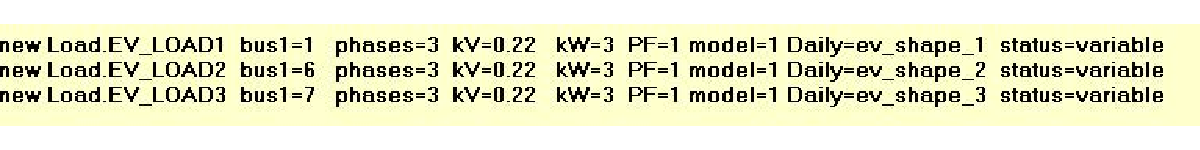
\includegraphics[width = \textwidth]{../Figures/code_ev.pdf}
    \end{figure}
\end{frame}

\begin{frame}
    \frametitle{EV profiles, N1, N6, N13}
    % \framesubtitle{EV profiles, N1, N6, N13}

    \begin{figure}
            \begin{tikzpicture}[baseline]
                \begin{axis}[
                xlabel={Period time [h]},
                ylabel near ticks,
                xlabel near ticks,
                ylabel={p.u.},
                % tick style = {line width = 0.5, color = lightgray, 
                %     major tick length=4pt,minor tick length=2pt,
                %     minor x tick num = 3, minor y tick num =1},
                % tick label style = {font=\small, xtick distance=1}
                    % xticklabels={00:00, 00:00, 04:00, 08:00, 12:00, 16:00, 20:00},
                % label style = {},
                legend style = {font=\footnotesize, at={(0.99,0.98)}, 
                    legend cell align=left, line width=0.5pt, draw=lightgray},
                % % legend entries={High PV, Medium PV, Low PV, High load, Medium load, Low load},
                % ymin=115, ymax=135,
                xmin=1, xmax=24,
                width=12cm,
                height=7.5cm,
                axis line style = {lightgray, line width = 0.5pt},
                cycle multi list={
                black\nextlist
                linestyles
                }
                ]
                \addplot  table 
                    [col sep=comma, y=P1] {../Data/profiles_ev.dat};
                \addlegendentry[]{P1}
                \addplot  table 
                    [col sep=comma, y=P2] {../Data/profiles_ev.dat};
                \addlegendentry[]{P2}
                \addplot  table 
                    [col sep=comma, y=P3] {../Data/profiles_ev.dat};
                \addlegendentry[]{P3}

                % \only<2->{\addplot  table 
                %     [col sep=comma, x=h, y=pd_m] {../Data/pv_pd.dat};
                %     \addlegendentry{Medium load}}
                % \only<3->{\addplot  table 
                %     [col sep=comma, x=h, y=pd_l] {../Data/pv_pd.dat};
                %     \addlegendentry{Low load}}
            
                % \only<4->{\addplot  table 
                %     [col sep=comma, x=h, y=pv_m] {../Data/pv_pd.dat};
                %     \addlegendentry{Medium PV}}
                % \only<5->{\addplot  table 
                %     [col sep=comma, x=h, y=pv_l] {../Data/pv_pd.dat};
                %     \addlegendentry{Low PV}}
                \end{axis}
            \end{tikzpicture} 
            \caption{EV profiles.}
    \end{figure}

\end{frame}

\section{Results}

\begin{frame}
    \frametitle{Results}
    \framesubtitle{Voltage profiles for Node 1}

    \begin{figure}
            \begin{tikzpicture}[baseline]
                \begin{axis}[
                xlabel={Period time [h]},
                ylabel near ticks,
                xlabel near ticks,
                ylabel={Voltage [V]},
                % tick style = {line width = 0.5, color = lightgray, 
                %     major tick length=4pt,minor tick length=2pt,
                %     minor x tick num = 3, minor y tick num =1},
                % tick label style = {font=\small, xtick distance=4, 
                %     xticklabels={00:00, 00:00, 04:00, 08:00, 12:00, 16:00, 20:00}},
                % label style = {},
                legend style = {font=\footnotesize, at={(0.99,0.98)}, 
                    legend cell align=left, line width=0.5pt, draw=lightgray},
                % % legend entries={High PV, Medium PV, Low PV, High load, Medium load, Low load},
                ymin=115, ymax=135,
                % % xmin=0, xmax=23,
                width=12cm,
                height=7.5cm,
                % axis line style = {lightgray, line width = 0.5pt},
                % cycle multi list={
                % black, gray\nextlist
                % linestyles
                % }
                ]
                \addplot  table 
                    [col sep=comma, y=V1] {../Data/n1_base.dat};
                \addlegendentry[]{$V_{123}$}
                \addplot  table 
                    [col sep=comma, y=V2] {../Data/n1_e.dat};
                \addlegendentry[]{$V_{123}^{\text{EVs}}$}
                % \addplot  table 
                %     [col sep=comma, y=V3] {../Data/n1_base.dat};
                % \addlegendentry[]{V1}
                \addplot  table 
                    [col sep=comma, y=Vmin] {../Data/n1_base.dat}; 
                \addlegendentry{$V_{min}$}     
                \addplot  table 
                    [col sep=comma, y=Vmax] {../Data/n1_base.dat}; 
                \addlegendentry{$V_{max}$}     
                % \only<2->
                % \only<3->{\addplot  table 
                %     [col sep=comma, x=h, y=pd_l] {../Data/pv_pd.dat};
                %     \addlegendentry{Low load}}
            
                % \only<4->{\addplot  table 
                %     [col sep=comma, x=h, y=pv_m] {../Data/pv_pd.dat};
                %     \addlegendentry{Medium PV}}
                % \only<5->{\addplot  table 
                %     [col sep=comma, x=h, y=pv_l] {../Data/pv_pd.dat};
                %     \addlegendentry{Low PV}}
                \end{axis}
            \end{tikzpicture} 
            \caption{Voltage profiles for the N1 (House recharge).}
    \end{figure}

\end{frame}

\begin{frame}
    \frametitle{Results}
    \framesubtitle{Voltage profiles for Node 6 (Office recharge).}

    \begin{figure}
            \begin{tikzpicture}[baseline]
                \begin{axis}[
                xlabel={Period time [h]},
                ylabel near ticks,
                xlabel near ticks,
                ylabel={Voltage [V]},
                % tick style = {line width = 0.5, color = lightgray, 
                %     major tick length=4pt,minor tick length=2pt,
                %     minor x tick num = 3, minor y tick num =1},
                % tick label style = {font=\small, xtick distance=4, 
                %     xticklabels={00:00, 00:00, 04:00, 08:00, 12:00, 16:00, 20:00}},
                % label style = {},
                legend style = {font=\footnotesize, at={(0.99,0.98)}, 
                    legend cell align=left, line width=0.5pt, draw=lightgray},
                % % legend entries={High PV, Medium PV, Low PV, High load, Medium load, Low load},
                ymin=115, ymax=135,
                % % xmin=0, xmax=23,
                width=12cm,
                height=7.5cm,
                % axis line style = {lightgray, line width = 0.5pt},
                % cycle multi list={
                % black, gray\nextlist
                % linestyles
                % }
                ]
                \addplot  table 
                    [col sep=comma, y=V1] {../Data/n6_base.dat};
                \addlegendentry[]{$V_{123}$}
                \addplot  table 
                    [col sep=comma, y=V2] {../Data/n6_e.dat};
                \addlegendentry[]{$V_{123}^{\text{EVs}}$}
                % \addplot  table 
                %     [col sep=comma, y=V3] {../Data/n1_base.dat};
                % \addlegendentry[]{V1}
                \addplot  table 
                    [col sep=comma, y=Vmin] {../Data/n6_base.dat}; 
                \addlegendentry{$V_{min}$}     
                \addplot  table 
                    [col sep=comma, y=Vmax] {../Data/n6_base.dat}; 
                \addlegendentry{$V_{max}$}     
                % \only<2->{\addplot  table 
                %     [col sep=comma, x=h, y=pd_m] {../Data/pv_pd.dat};
                %     \addlegendentry{Medium load}}
                % \only<3->{\addplot  table 
                %     [col sep=comma, x=h, y=pd_l] {../Data/pv_pd.dat};
                %     \addlegendentry{Low load}}
            
                % \only<4->{\addplot  table 
                %     [col sep=comma, x=h, y=pv_m] {../Data/pv_pd.dat};
                %     \addlegendentry{Medium PV}}
                % \only<5->{\addplot  table 
                %     [col sep=comma, x=h, y=pv_l] {../Data/pv_pd.dat};
                %     \addlegendentry{Low PV}}
                \end{axis}
            \end{tikzpicture} 
            \caption{Voltage profiles for the N6.}
    \end{figure}

\end{frame}

\begin{frame}
    \frametitle{Results}
    \framesubtitle{Voltage profiles for Node 13 (Fast recharge).}

    \begin{figure}
            \begin{tikzpicture}[baseline]
                \begin{axis}[
                xlabel={Period time [h]},
                ylabel near ticks,
                xlabel near ticks,
                ylabel={Voltage [V]},
                % tick style = {line width = 0.5, color = lightgray, 
                %     major tick length=4pt,minor tick length=2pt,
                %     minor x tick num = 3, minor y tick num =1},
                % tick label style = {font=\small, xtick distance=4, 
                %     xticklabels={00:00, 00:00, 04:00, 08:00, 12:00, 16:00, 20:00}},
                % label style = {},
                legend style = {font=\footnotesize, at={(0.99,0.98)}, 
                    legend cell align=left, line width=0.5pt, draw=lightgray},
                % % legend entries={High PV, Medium PV, Low PV, High load, Medium load, Low load},
                ymin=115, ymax=135,
                % % xmin=0, xmax=23,
                width=12cm,
                height=7.5cm,
                % axis line style = {lightgray, line width = 0.5pt},
                % cycle multi list={
                % black, gray\nextlist
                % linestyles
                % }
                ]
                \addplot  table 
                    [col sep=comma, y=V1] {../Data/n13_base.dat};
                \addlegendentry[]{$V_{123}$}
                \addplot  table 
                    [col sep=comma, y=V2] {../Data/n13_e.dat};
                \addlegendentry[]{$V_{123}^{\text{EVs}}$}
                % \addplot  table 
                %     [col sep=comma, y=V3] {../Data/n1_base.dat};
                % \addlegendentry[]{V1}
                \addplot  table 
                    [col sep=comma, y=Vmin] {../Data/n13_base.dat}; 
                \addlegendentry{$V_{min}$}     
                \addplot  table 
                    [col sep=comma, y=Vmax] {../Data/n13_base.dat}; 
                \addlegendentry{$V_{max}$}     
                % \only<2->{\addplot  table 
                %     [col sep=comma, x=h, y=pd_m] {../Data/pv_pd.dat};
                %     \addlegendentry{Medium load}}
                % \only<3->{\addplot  table 
                %     [col sep=comma, x=h, y=pd_l] {../Data/pv_pd.dat};
                %     \addlegendentry{Low load}}
            
                % \only<4->{\addplot  table 
                %     [col sep=comma, x=h, y=pv_m] {../Data/pv_pd.dat};
                %     \addlegendentry{Medium PV}}
                % \only<5->{\addplot  table 
                %     [col sep=comma, x=h, y=pv_l] {../Data/pv_pd.dat};
                %     \addlegendentry{Low PV}}
                \end{axis}
            \end{tikzpicture} 
            \caption{Voltage profiles for the N13.}
    \end{figure}

\end{frame}


% \begin{frame}
%     \frametitle{Correction of the voltage magnitude}
%     \framesubtitle{Voltage profiles for Node 1}

%     \begin{figure}
%             \begin{tikzpicture}[baseline]
%                 \begin{axis}[
%                 xlabel={Period time [h]},
%                 ylabel near ticks,
%                 xlabel near ticks,
%                 ylabel={Voltage [V]},
%                 % tick style = {line width = 0.5, color = lightgray, 
%                 %     major tick length=4pt,minor tick length=2pt,
%                 %     minor x tick num = 3, minor y tick num =1},
%                 % tick label style = {font=\small, xtick distance=4, 
%                 %     xticklabels={00:00, 00:00, 04:00, 08:00, 12:00, 16:00, 20:00}},
%                 % label style = {},
%                 legend style = {font=\footnotesize, at={(0.99,0.98)}, 
%                     legend cell align=left, line width=0.5pt, draw=lightgray},
%                 % % legend entries={High PV, Medium PV, Low PV, High load, Medium load, Low load},
%                 ymin=115, ymax=135,
%                 % % xmin=0, xmax=23,
%                 width=12cm,
%                 height=7.5cm,
%                 % axis line style = {lightgray, line width = 0.5pt},
%                 % cycle multi list={
%                 % black, gray\nextlist
%                 % linestyles
%                 % }
%                 ]
%                 \addplot  table 
%                     [col sep=comma, y=V1] {../Data/n1_base.dat};
%                 \addlegendentry[]{$V_{123}$}
%                 \addplot  table 
%                     [col sep=comma, y=V2] {../Data/n1_e.dat};
%                 \addlegendentry[]{$V_{123}^{\text{EVs}}$}
%                 % \addplot  table 
%                 %     [col sep=comma, y=V3] {../Data/n1_base.dat};
%                 % \addlegendentry[]{V1}
%                 \addplot  table 
%                     [col sep=comma, y=Vmin] {../Data/n1_base.dat}; 
%                 \addlegendentry{$V_{min}$}     
%                 \addplot  table 
%                     [col sep=comma, y=Vmax] {../Data/n1_base.dat}; 
%                 \addlegendentry{$V_{max}$}     
%                 % \only<2->
%                 % \only<3->{\addplot  table 
%                 %     [col sep=comma, x=h, y=pd_l] {../Data/pv_pd.dat};
%                 %     \addlegendentry{Low load}}
            
%                 % \only<4->{\addplot  table 
%                 %     [col sep=comma, x=h, y=pv_m] {../Data/pv_pd.dat};
%                 %     \addlegendentry{Medium PV}}
%                 % \only<5->{\addplot  table 
%                 %     [col sep=comma, x=h, y=pv_l] {../Data/pv_pd.dat};
%                 %     \addlegendentry{Low PV}}
%                 \end{axis}
%             \end{tikzpicture} 
%             \caption{Voltage profiles for the N1.}
%     \end{figure}

% \end{frame}

% \begin{frame}
%     \frametitle{Correction of the voltage magnitude}
%     \framesubtitle{Voltage profiles for Node 6}

%     \begin{figure}
%             \begin{tikzpicture}[baseline]
%                 \begin{axis}[
%                 xlabel={Period time [h]},
%                 ylabel near ticks,
%                 xlabel near ticks,
%                 ylabel={Voltage [V]},
%                 % tick style = {line width = 0.5, color = lightgray, 
%                 %     major tick length=4pt,minor tick length=2pt,
%                 %     minor x tick num = 3, minor y tick num =1},
%                 % tick label style = {font=\small, xtick distance=4, 
%                 %     xticklabels={00:00, 00:00, 04:00, 08:00, 12:00, 16:00, 20:00}},
%                 % label style = {},
%                 legend style = {font=\footnotesize, at={(0.99,0.98)}, 
%                     legend cell align=left, line width=0.5pt, draw=lightgray},
%                 % % legend entries={High PV, Medium PV, Low PV, High load, Medium load, Low load},
%                 ymin=115, ymax=135,
%                 % % xmin=0, xmax=23,
%                 width=12cm,
%                 height=7.5cm,
%                 % axis line style = {lightgray, line width = 0.5pt},
%                 % cycle multi list={
%                 % black, gray\nextlist
%                 % linestyles
%                 % }
%                 ]
%                 \addplot  table 
%                     [col sep=comma, y=V1] {../Data/n6_base.dat};
%                 \addlegendentry[]{$V_{123}$}
%                 \addplot  table 
%                     [col sep=comma, y=V2] {../Data/n6_e.dat};
%                 \addlegendentry[]{$V_{123}^{\text{EVs}}$}
%                 % \addplot  table 
%                 %     [col sep=comma, y=V3] {../Data/n1_base.dat};
%                 % \addlegendentry[]{V1}
%                 \addplot  table 
%                     [col sep=comma, y=Vmin] {../Data/n6_base.dat}; 
%                 \addlegendentry{$V_{min}$}     
%                 \addplot  table 
%                     [col sep=comma, y=Vmax] {../Data/n6_base.dat}; 
%                 \addlegendentry{$V_{max}$}     
%                 % \only<2->{\addplot  table 
%                 %     [col sep=comma, x=h, y=pd_m] {../Data/pv_pd.dat};
%                 %     \addlegendentry{Medium load}}
%                 % \only<3->{\addplot  table 
%                 %     [col sep=comma, x=h, y=pd_l] {../Data/pv_pd.dat};
%                 %     \addlegendentry{Low load}}
            
%                 % \only<4->{\addplot  table 
%                 %     [col sep=comma, x=h, y=pv_m] {../Data/pv_pd.dat};
%                 %     \addlegendentry{Medium PV}}
%                 % \only<5->{\addplot  table 
%                 %     [col sep=comma, x=h, y=pv_l] {../Data/pv_pd.dat};
%                 %     \addlegendentry{Low PV}}
%                 \end{axis}
%             \end{tikzpicture} 
%             \caption{Voltage profiles for the N6.}
%     \end{figure}

% \end{frame}

\begin{frame}
    \frametitle{Correction of the voltage magnitude}
    \framesubtitle{Charging power reduced from 3 kW to 1 kW}

    \begin{figure}
            \begin{tikzpicture}[baseline]
                \begin{axis}[
                xlabel={Period time [h]},
                ylabel near ticks,
                xlabel near ticks,
                ylabel={Voltage [V]},
                % tick style = {line width = 0.5, color = lightgray, 
                %     major tick length=4pt,minor tick length=2pt,
                %     minor x tick num = 3, minor y tick num =1},
                % tick label style = {font=\small, xtick distance=4, 
                %     xticklabels={00:00, 00:00, 04:00, 08:00, 12:00, 16:00, 20:00}},
                % label style = {},
                legend style = {font=\footnotesize, at={(0.99,0.98)}, 
                    legend cell align=left, line width=0.5pt, draw=lightgray},
                % % legend entries={High PV, Medium PV, Low PV, High load, Medium load, Low load},
                ymin=115, ymax=135,
                % % xmin=0, xmax=23,
                width=12cm,
                height=7.5cm,
                % axis line style = {lightgray, line width = 0.5pt},
                % cycle multi list={
                % black, gray\nextlist
                % linestyles
                % }
                ]
                \addplot  table 
                    [col sep=comma, y=V3] {../Data/n13_e_c.dat};
                \addlegendentry[]{After - $V_{123}^{\text{EVs}}$}
                \addplot  table 
                    [col sep=comma, y=V2] {../Data/n13_e.dat};
                \addlegendentry[]{Before - $V_{123}^{\text{EVs}}$}
                % \addplot  table 
                %     [col sep=comma, y=V3] {../Data/n1_base.dat};
                % \addlegendentry[]{V1}
                \addplot  table 
                    [col sep=comma, y=Vmin] {../Data/n13_base.dat}; 
                \addlegendentry{$V_{min}$}     
                \addplot  table 
                    [col sep=comma, y=Vmax] {../Data/n13_base.dat}; 
                \addlegendentry{$V_{max}$}     
                % \only<2->{\addplot  table 
                %     [col sep=comma, x=h, y=pd_m] {../Data/pv_pd.dat};
                %     \addlegendentry{Medium load}}
                % \only<3->{\addplot  table 
                %     [col sep=comma, x=h, y=pd_l] {../Data/pv_pd.dat};
                %     \addlegendentry{Low load}}
            
                % \only<4->{\addplot  table 
                %     [col sep=comma, x=h, y=pv_m] {../Data/pv_pd.dat};
                %     \addlegendentry{Medium PV}}
                % \only<5->{\addplot  table 
                %     [col sep=comma, x=h, y=pv_l] {../Data/pv_pd.dat};
                %     \addlegendentry{Low PV}}
                \end{axis}
            \end{tikzpicture} 
            \caption{Voltage profiles for the N13.}
    \end{figure}

\end{frame}


\begin{frame}
    \frametitle{AMT QU02 - SED022}
    \begin{figure}
        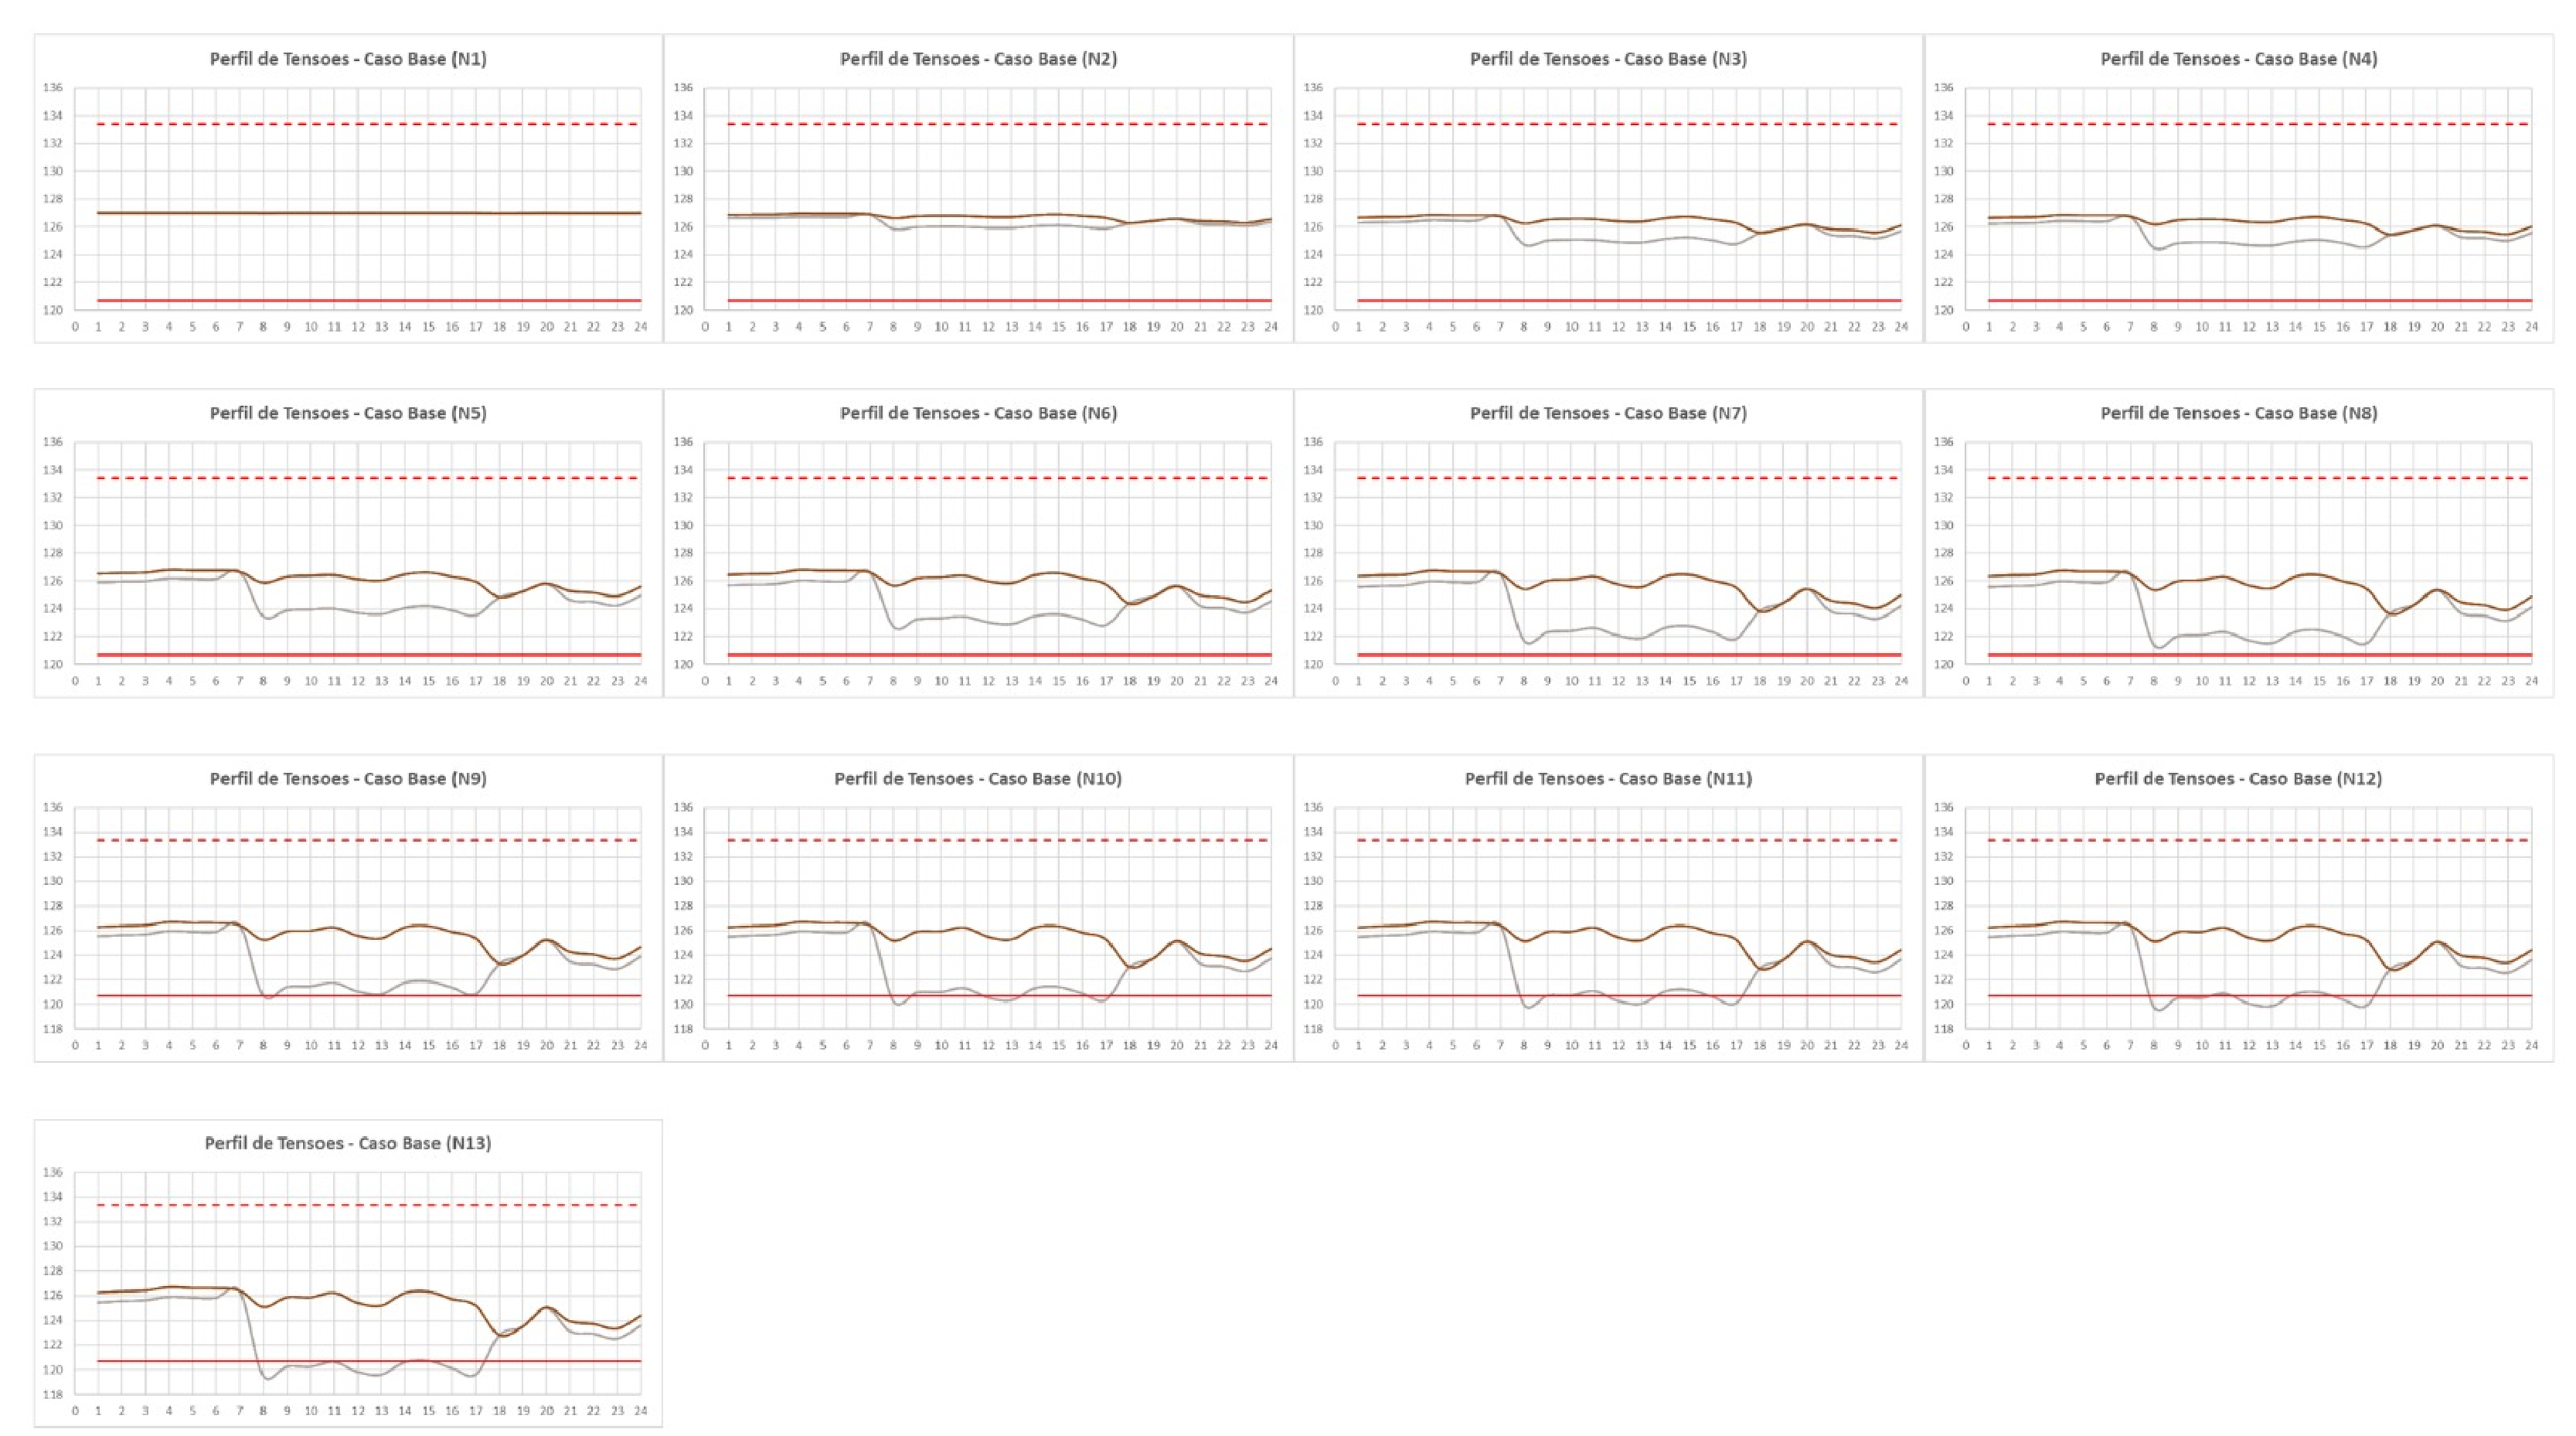
\includegraphics[width = \textwidth]{../Figures/allresults.pdf}
    \end{figure}
\end{frame}

\begin{frame}
    \frametitle{AMT QU02 - SED022}
    \begin{figure}
        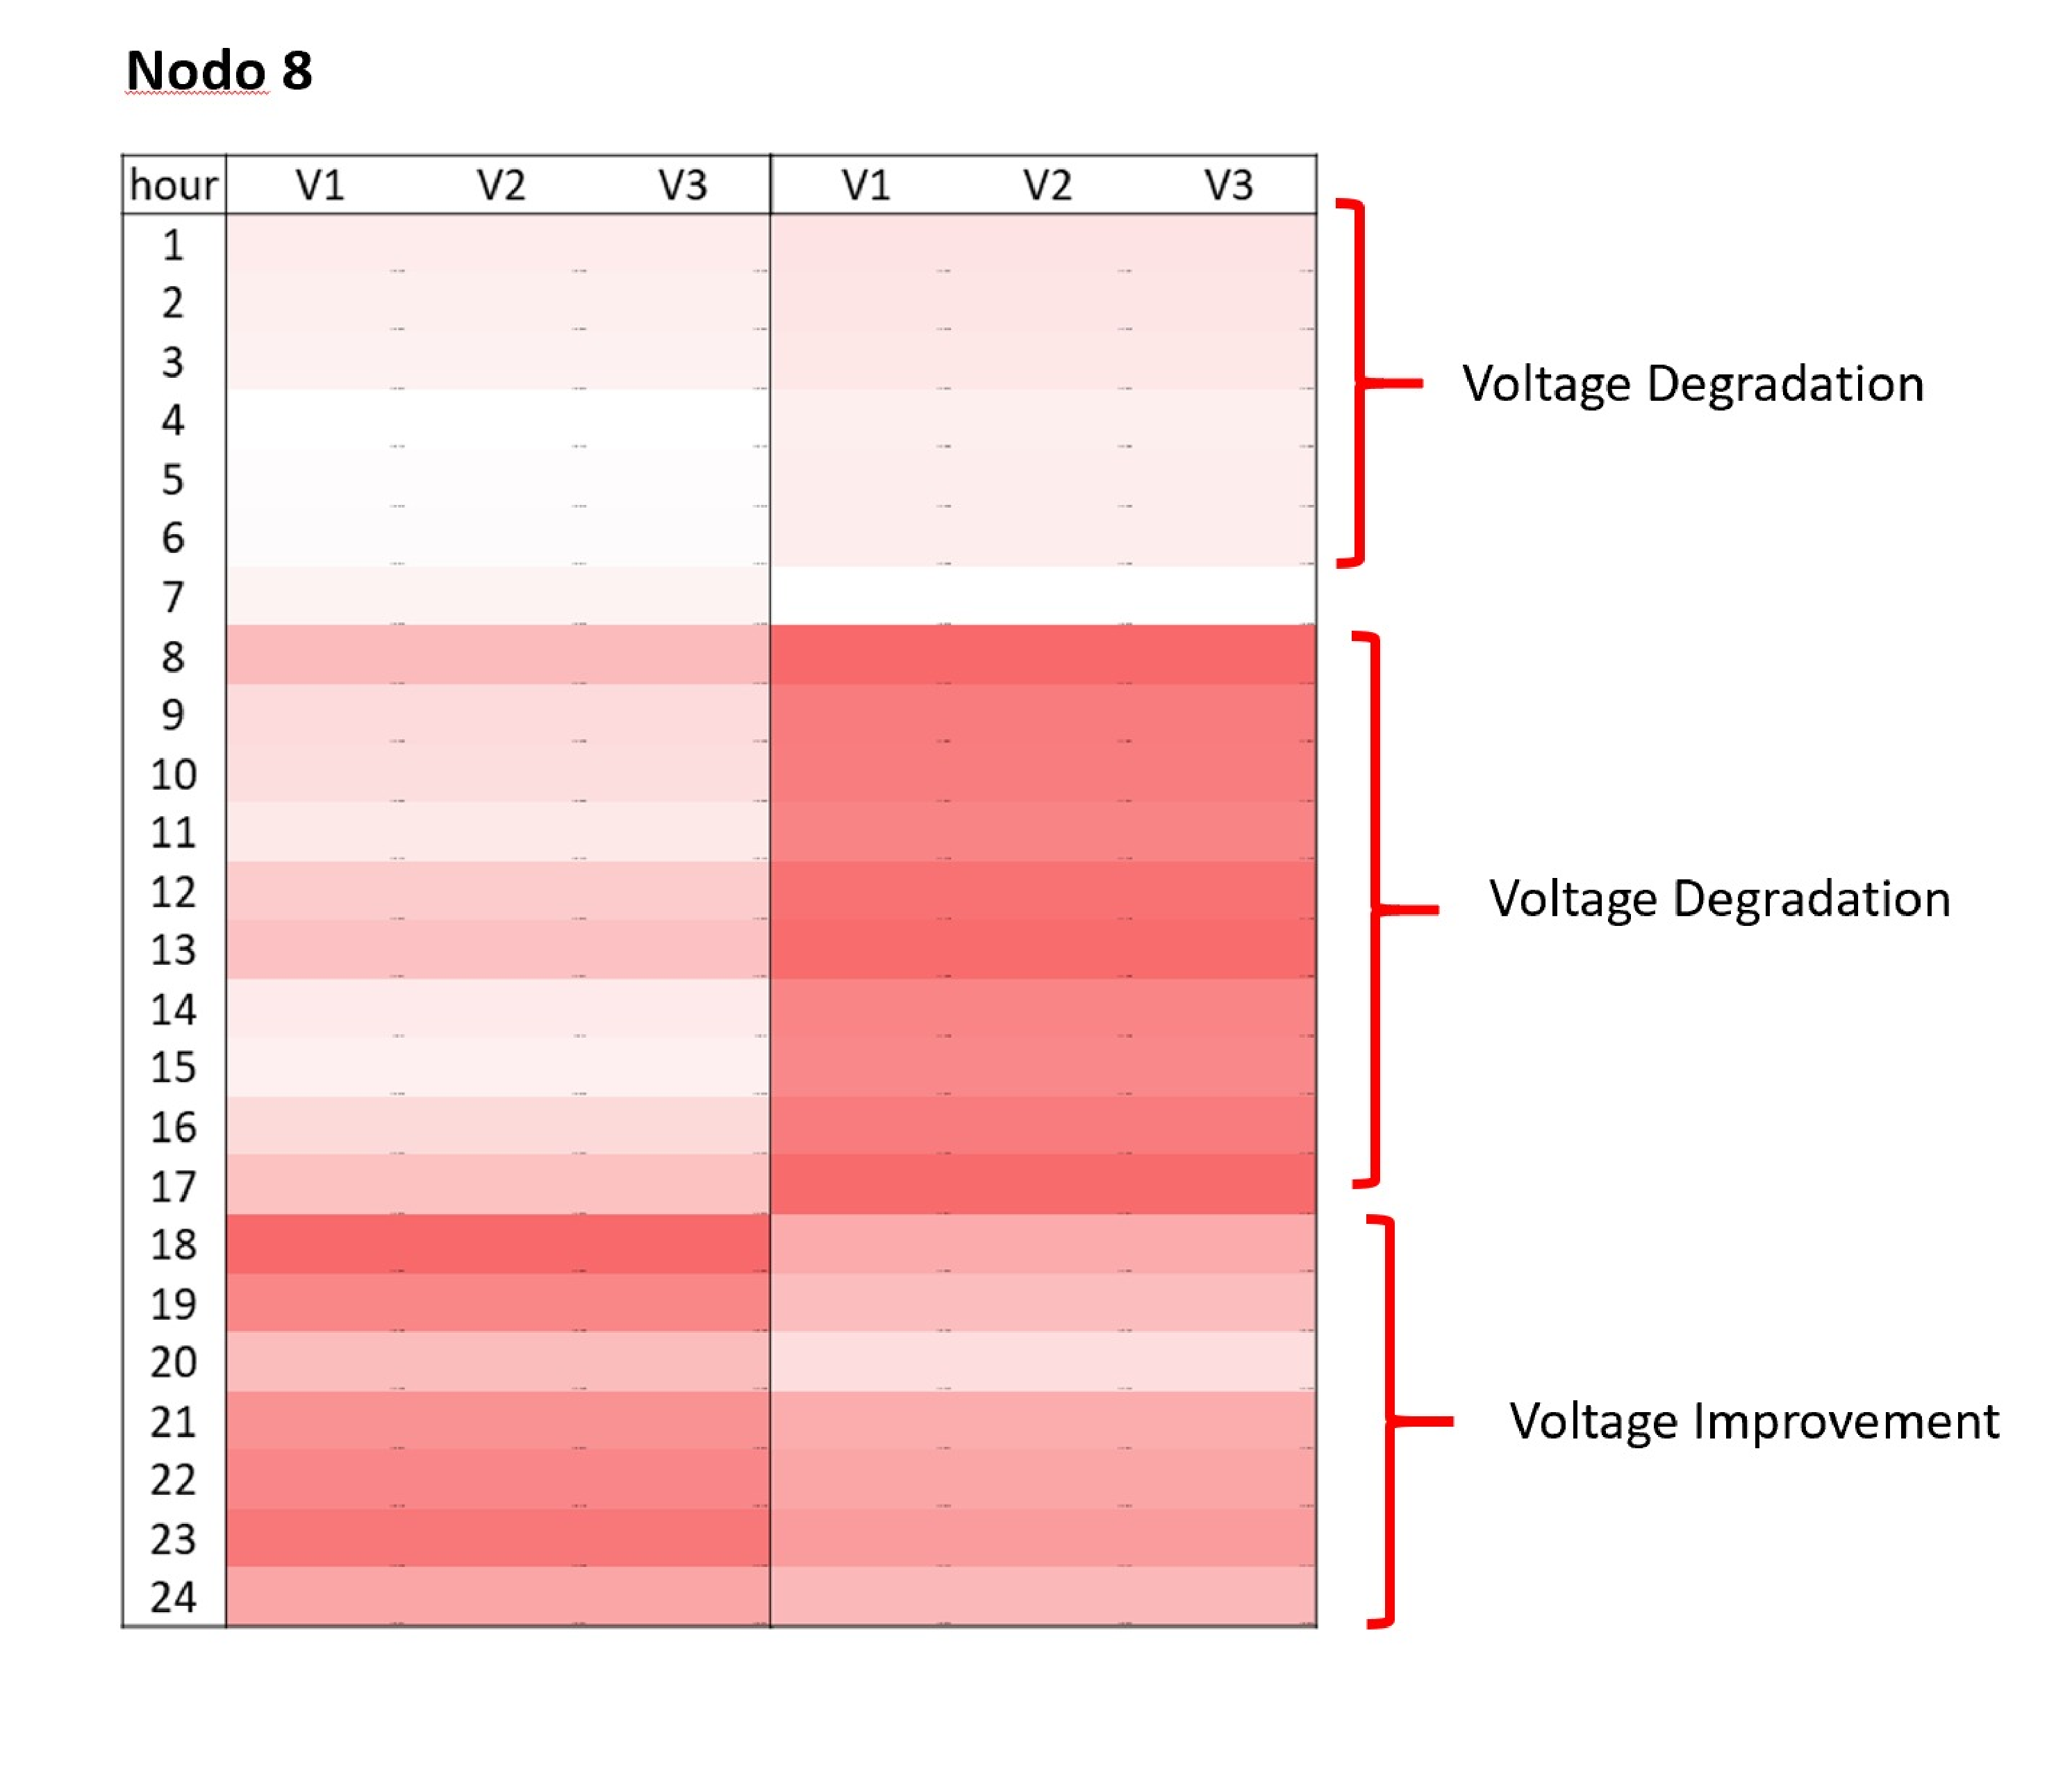
\includegraphics[width = \textheight]{../Figures/nodo8.pdf}
    \end{figure}
\end{frame}

\section{Conclusions}

\begin{frame}
    \frametitle{Conclusions}

    \begin{itemize}%[<+->]
        \item The distribution company lacks a systematized database, 
        making it difficult to manage data efficiently and conduct 
        accurate analysis.

        \item In some cases, the data showed inconsistencies, which 
        could affect the reliability of results and decision-making.

        \item The connection of electric vehicles causes voltage issues 
        in the grid, particularly at the busbars where fast charging 
        stations were installed. These issues need to be addressed to avoid 
        overloads or voltage drops that could impact grid stability.

        \item Real data demonstrated that the integration of EVs 
        into the grid requires a detailed study. Computational 
        tools like OpenDSS are essential for conducting accurate simulations 
        and assessing their impact on the network.

        \item OpenDSS is a versatile tool that supports detailed analysis 
        and allows for automation in generating multiple scenarios, making 
        it crucial for efficient planning and decision-making.


    \end{itemize}
\end{frame}


\begin{frame}
    \textbf{Thank you!}
\end{frame}
\end{document}
    